\documentclass[titlepage]{jsarticle}


% 数式
\usepackage{amsmath,amsfonts}
\usepackage{bm}
\usepackage{physics}
% 画像
\usepackage[dvipdfmx]{graphicx}
% ローマ数字
\usepackage{otf}
% 単位
\usepackage{siunitx}
% 表
\usepackage{multirow}
% コメント
\usepackage{comment}

\begin{document}

\title{物理学実験\ajRoman{2}レポート(分光測定3A)}
\author{05-211525 齋藤駿一 \\
  共同実験者:新居智将,河野匡}
\date{\today 提出}
\maketitle

\section{目的}
本実験では,分光測定技術の基礎を学び,実際に物質のエネルギー構造を探る.
具体的には,まず分光器の原理と使用法を学ぶ.
次に水素原子の発光スペクトルを測定する.
最後に半導体の光学応答を調べる.

\section{一日目:分光器の原理・測定装置の使用法}

\subsection{分光器の準備}
最初に,次の手順に沿って分光器の準備を行った.

まず,分光器の入射・出射スリットが閉じていることを確認した.
次に,分光器の出口に光電子増倍管を置き,\SI{-500}{V}の高電圧をかけた.
また,分光器の入口手前にレンズと水銀アルゴン光源を置いた.
このときレンズと光源の位置は,光源からの光がレンズを通り,入射スリットの位置に集光するように調整した.
その後,光電子増倍管の出力を電流電圧変換増幅器に繋いだ.
そのうえで,電流電圧変換増幅器の出力をオシロスコープに繋ぎ,分光器の入射・出射スリットを開いたときの波形をもとに,レンズの位置と向きを微調整した.

ただし,本実験全体を通して,光電子増倍管の出力電流は\SI{2}{nA}を超えないように注意した.
具体的には,電流電圧変換増幅器の出力をオシロスコープに適宜つないで,光電子増倍管の出力電圧を確認した.

\subsection{課題(a)}
まず分光器の入射・出射スリットのゼロ点を調べた.

\subsubsection{手法}
まず,電流電圧変換増幅器の出力をペンレコーダーに入力した.
この状態でレコーダーのペンを下ろすと,増幅器の出力に応じてペンが動いた.
そこで,入射・出射スリットの開閉を調整するマイクロメーターをある程度回して固定してから,分光器の入口で光を遮った.
このときペンが動けばスリットは開いており,動かなければスリットは閉じていると確認できる.
ここでは,マイクロメーターの値を変えながらこの測定を繰り返し,入射・出射スリットが開き始めるときのマイクロメーターの目盛りを調べた.
これを入射・出射スリットのマイクロメーターのゼロ点とし,これ以降のスリットの操作はこの結果を基準に行った.

\subsubsection{結果}
実験の結果,入射スリットのゼロ点は\SI{1}{\um},出射スリットのゼロ点は\SI{110}{\um}と分かった.

\subsection{課題(b)}
ここでは光源とレンズの間にNDフィルター(ND2,ND4,ND8の3種類)を入れ,これによる光電流の変化(ペンの位置の変化)を調べた.

\subsubsection{手法}
まず,NDフィルターを入れずに入射・出射スリットを開き,そのときの光電流をペンレコーダーで記録した.
次に,スリット直前のレンズの前方にNDフィルター(ND2)を入れ,そのときの光電流をペンレコーダーで記録した.
同様の操作をND4,ND8についても行った.
最後に,光を遮ったときの光電流も記録した.

\subsubsection{結果}
\begin{figure}[htbp]
  \centering
  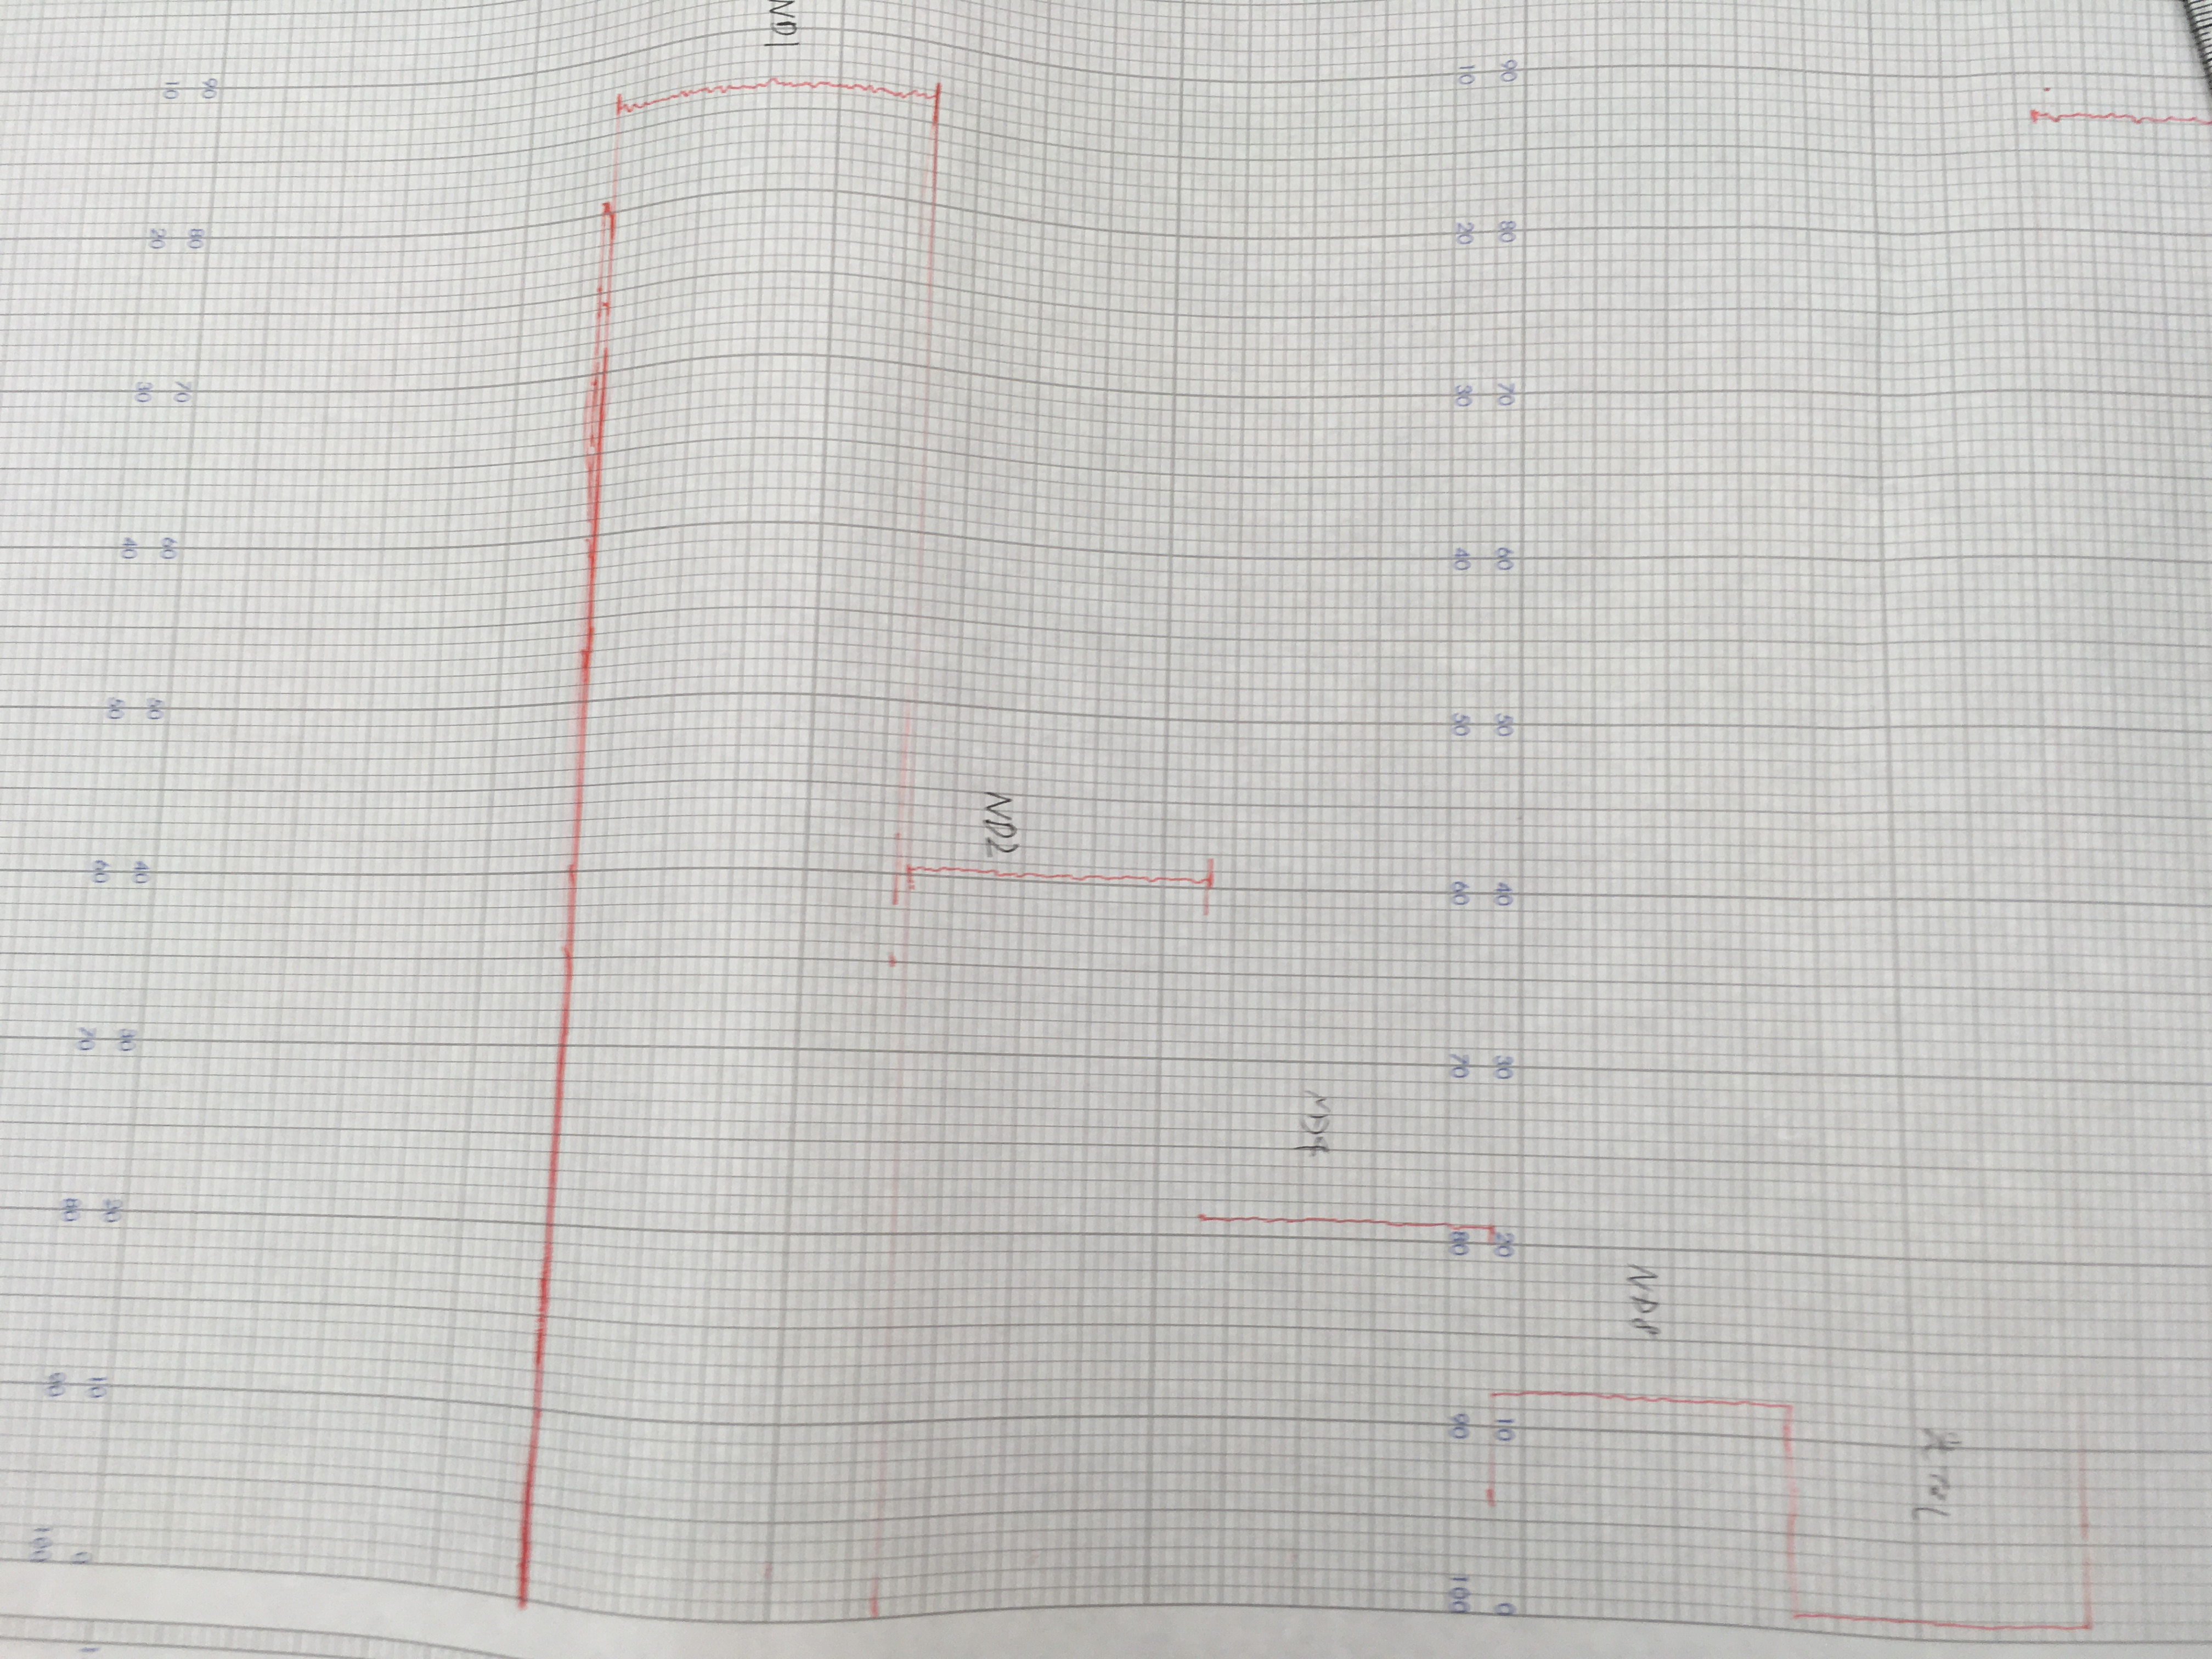
\includegraphics[width=10cm]{b_ND.JPG}
  \caption{NDフィルターを入れたときの光電流の変化(左からNDフィルターなし,ND2,ND4,ND8,光なし)}
  \label{fig:ND}
\end{figure}

\begin{table}[htbp]
  \centering
  \caption{NDフィルターを入れたときのペンの位置およびペンの振れ幅の比;ペンの位置は光を遮ったときを基準とし,ペンの振れ幅の比はフィルターを置かなかったときを基準とした.}
  \label{tab:ND}
  \begin{tabular}{c|cc}
    フィルター & ペンの位置(mm) & ペンの振れ幅の比 \\
    \hline\hline
    なし & 171 & 1(基準) \\
    ND2 & 79 & 0.46 \\
    ND4 & 40 & 0.23\\
    ND8 & 22 & 0.13\\
    \hline
  \end{tabular}
\end{table}

実験の結果,図\ref{fig:ND}のようにペンが動いた.
光を遮ったときのペンの位置を基準にとると,ペンの位置は表\ref{tab:ND}のようになった.
また,フィルターを置かなかったときのペンの位置(振れ幅)に対して,フィルターを置いたときのペンの位置(振れ幅)の割合を計算した(同表).
その結果,ND2とND4はいずれも理論値(それぞれ0.50,0.25)よりも若干小さい値となった.

\subsection{課題(c)}
ここでは,スリットの縦幅・横幅をわずかに開いたときに光源から得られる輝線のスペクトル幅を求めた.

\subsubsection{手法}
まず,入射スリットと出射スリットをともに\SI{10}{\um}だけ開いた.
次に,分光器の波長を\SI{434}{\nm}に合わせた.
そこから\SI{435}{\nm}まで分光器を動かし,輝線のスペクトルをペンレコーダーで記録した\footnote{後で見るように,これは実際の波長とは異なる.実際に測定した波長の領域は,課題(g)で導く波長の較正直線をもとに考えると,\SI{435.7}{\nm}~\SI{436.7}{\nm}となる.}.
ここで,ペンレコーダーの波長駆動速度は\SI{6}{\nm\per\min},CHART SPEEDは\SI{500}{\mm\per\min}に設定した.
その後,得られたスペクトルの幅(半値全幅)を求めた.

\subsubsection{結果}
\begin{figure}[htbp]
  \centering
  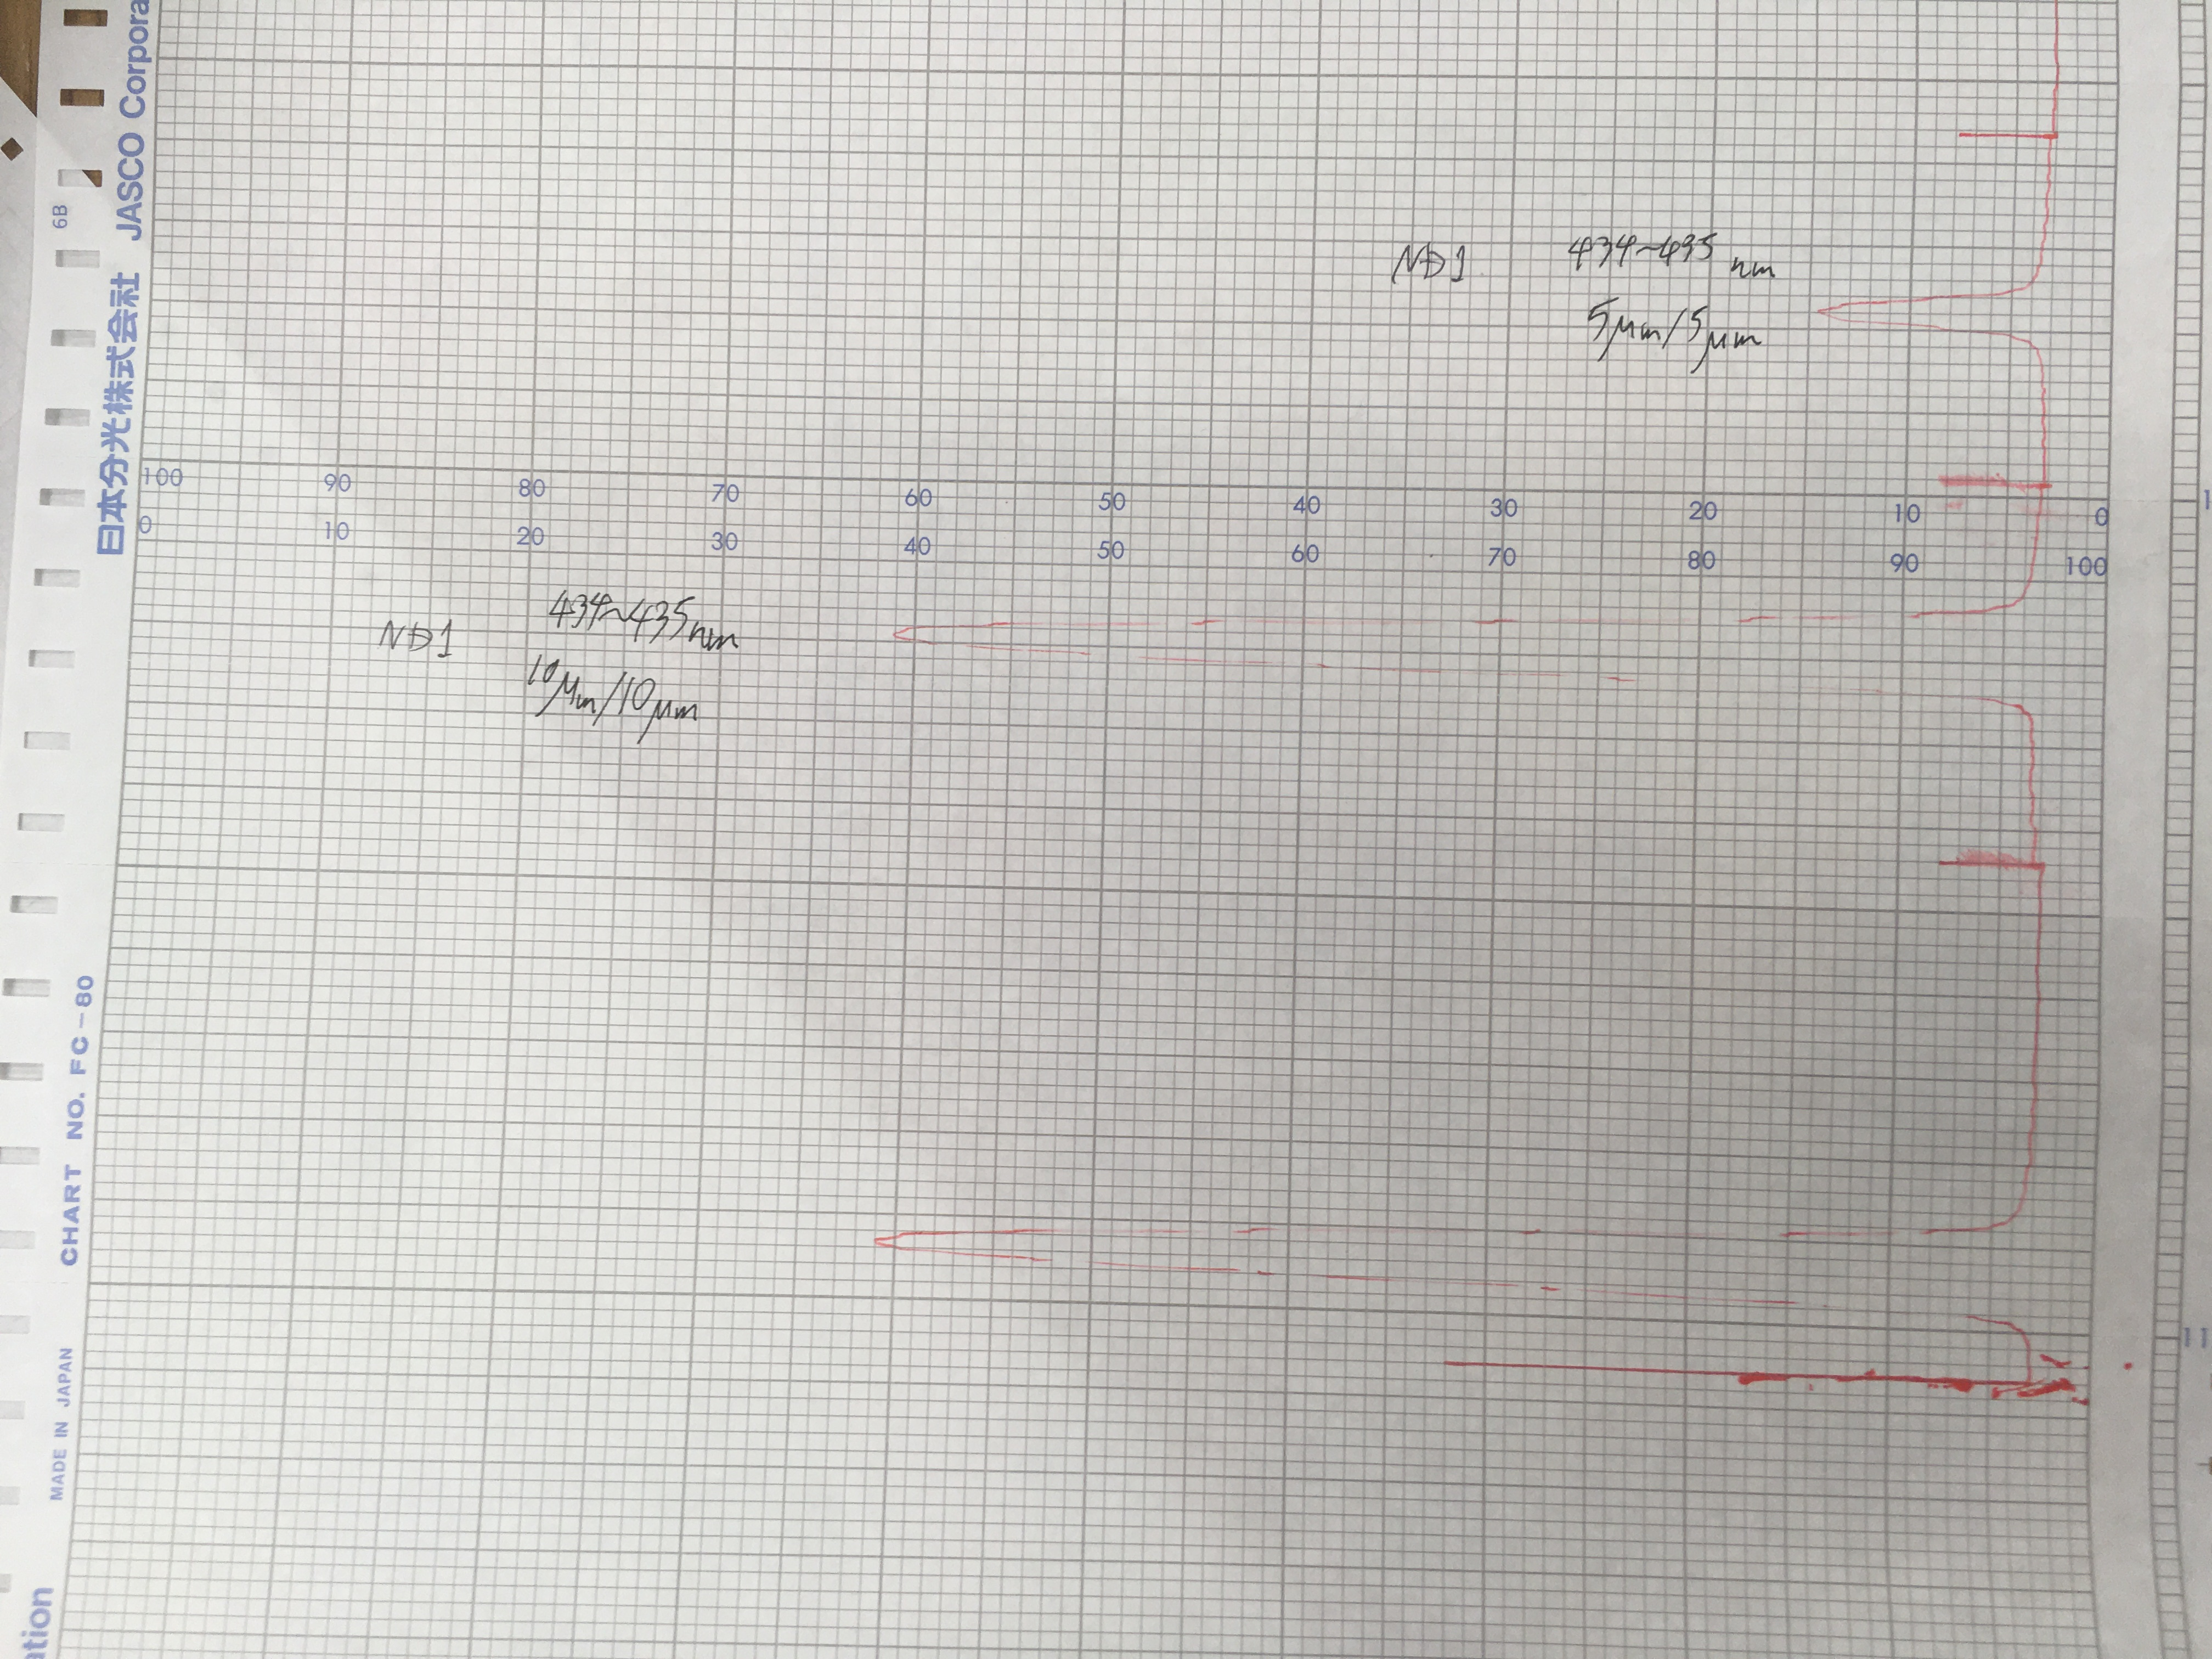
\includegraphics[width=10cm]{c_delta_min.JPG}
  \caption{水銀アルゴン光源の波長\SI{436}{\nm}付近のスペクトル(図中央).ただし,入射スリット幅\SI{10}{\um},出射スリット幅\SI{10}{\um}とした.}
  \label{fig:delta_min}
\end{figure}

実験の結果,ペンレコーダーの記録したスペクトルの半値全幅は\SI{6}{\mm}であった.
これとペンレコーダーの設定から,スペクトル幅は\SI{72}{\pm}と求まった.

\subsection{課題(d)}
ここでは,スリットの縦幅をなるべく小さくしたままスリットの横幅を変えてスペクトルを計測した.
そして,スリットの横幅$\Delta x$と得られたスペクトル幅$\Delta \lambda$の関係を調べた.

\subsubsection{手法}
まず,出射スリットの幅を\SI{10}{\um}に調整した.
次に,入射スリットの横幅$\Delta x$を\SI{5}{\um},\SI{20}{\um},\SI{30}{\um},\SI{40}{\um},\SI{50}{\um},\SI{100}{\um},\SI{150}{\um},\SI{200}{\um}に調整して,それぞれの場合について課題(c)のときとまったく同様にスペクトルをペンレコーダーで計測した.
この結果をもとに,スペクトルの幅(半値全幅)を求めた.
また,課題(c)で測定した入射スリットの横幅\SI{10}{\um}の場合のスペクトル幅も合わせて,入射スリットの横幅$\Delta x$とスペクトル幅$\Delta\lambda$の関係をプロットした.

\subsubsection{結果}

\begin{table}[htbp]
  \centering
  \caption{入射スリットの横幅$\Delta x$とペンレコーダー上のスペクトル幅の関係}
  \label{tab:spectrum_width}
  \begin{tabular}{c|c}
    入射スリットの横幅(\si{\um}) & ペンレコーダー上のスペクトル幅(\si{\mm})\\
    \hline\hline
    5 & 5\\
    10 & 6\\
    20 & 6\\
    30 & 8\\
    40 & 9\\
    50 & 12\\
    100 & 26\\
    150 & 36\\
    200 & 47\\
    \hline
  \end{tabular}
\end{table}

\begin{figure}[htbp]
  \centering
  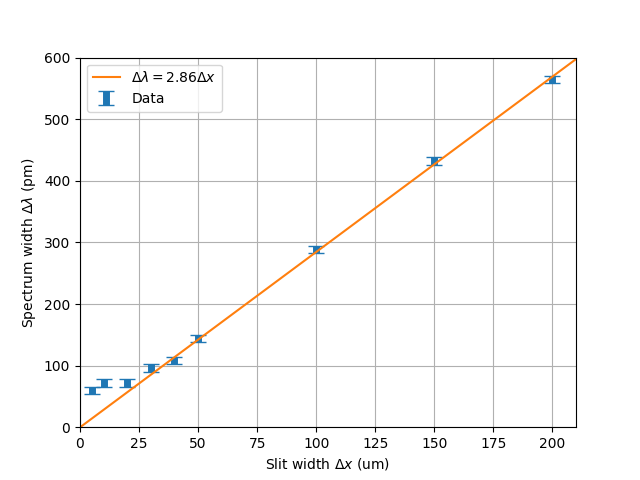
\includegraphics[width=10cm]{spectrum_width.png}
  \caption{出射スリットの幅を\SI{10}{\um}としたときの,入射スリットの横幅$\Delta x$とスペクトル幅$\Delta\lambda$の関係;誤差棒は,ペンレコーダー上のスペクトル幅に\SI{0.5}{\mm}の読み取り誤差があると考えて算出した.また,左から5番目以降のデータを用いて線形フィッティングを行った結果をオレンジ色で示す.}
  \label{fig:spectrum_width}
\end{figure}

実験の結果,入射スリットの横幅とペンレコーダー上のスペクトル幅の関係は表\ref{tab:spectrum_width}のようになり,このスペクトル幅を実際の波長に換算してプロットすると図\ref{fig:spectrum_width}のようになった.
図\ref{fig:spectrum_width}より,スリットの横幅が約\SI{50}{\um}より大きいところでは,スリットの横幅とスペクトル幅がほぼ比例していた.
一方,それより小さいスリット幅では,スペクトル幅は\SI{60}{\pm}~\SI{70}{\pm}で一定となり,それより小さくはならなかった.

\begin{figure}[htbp]
  \centering
  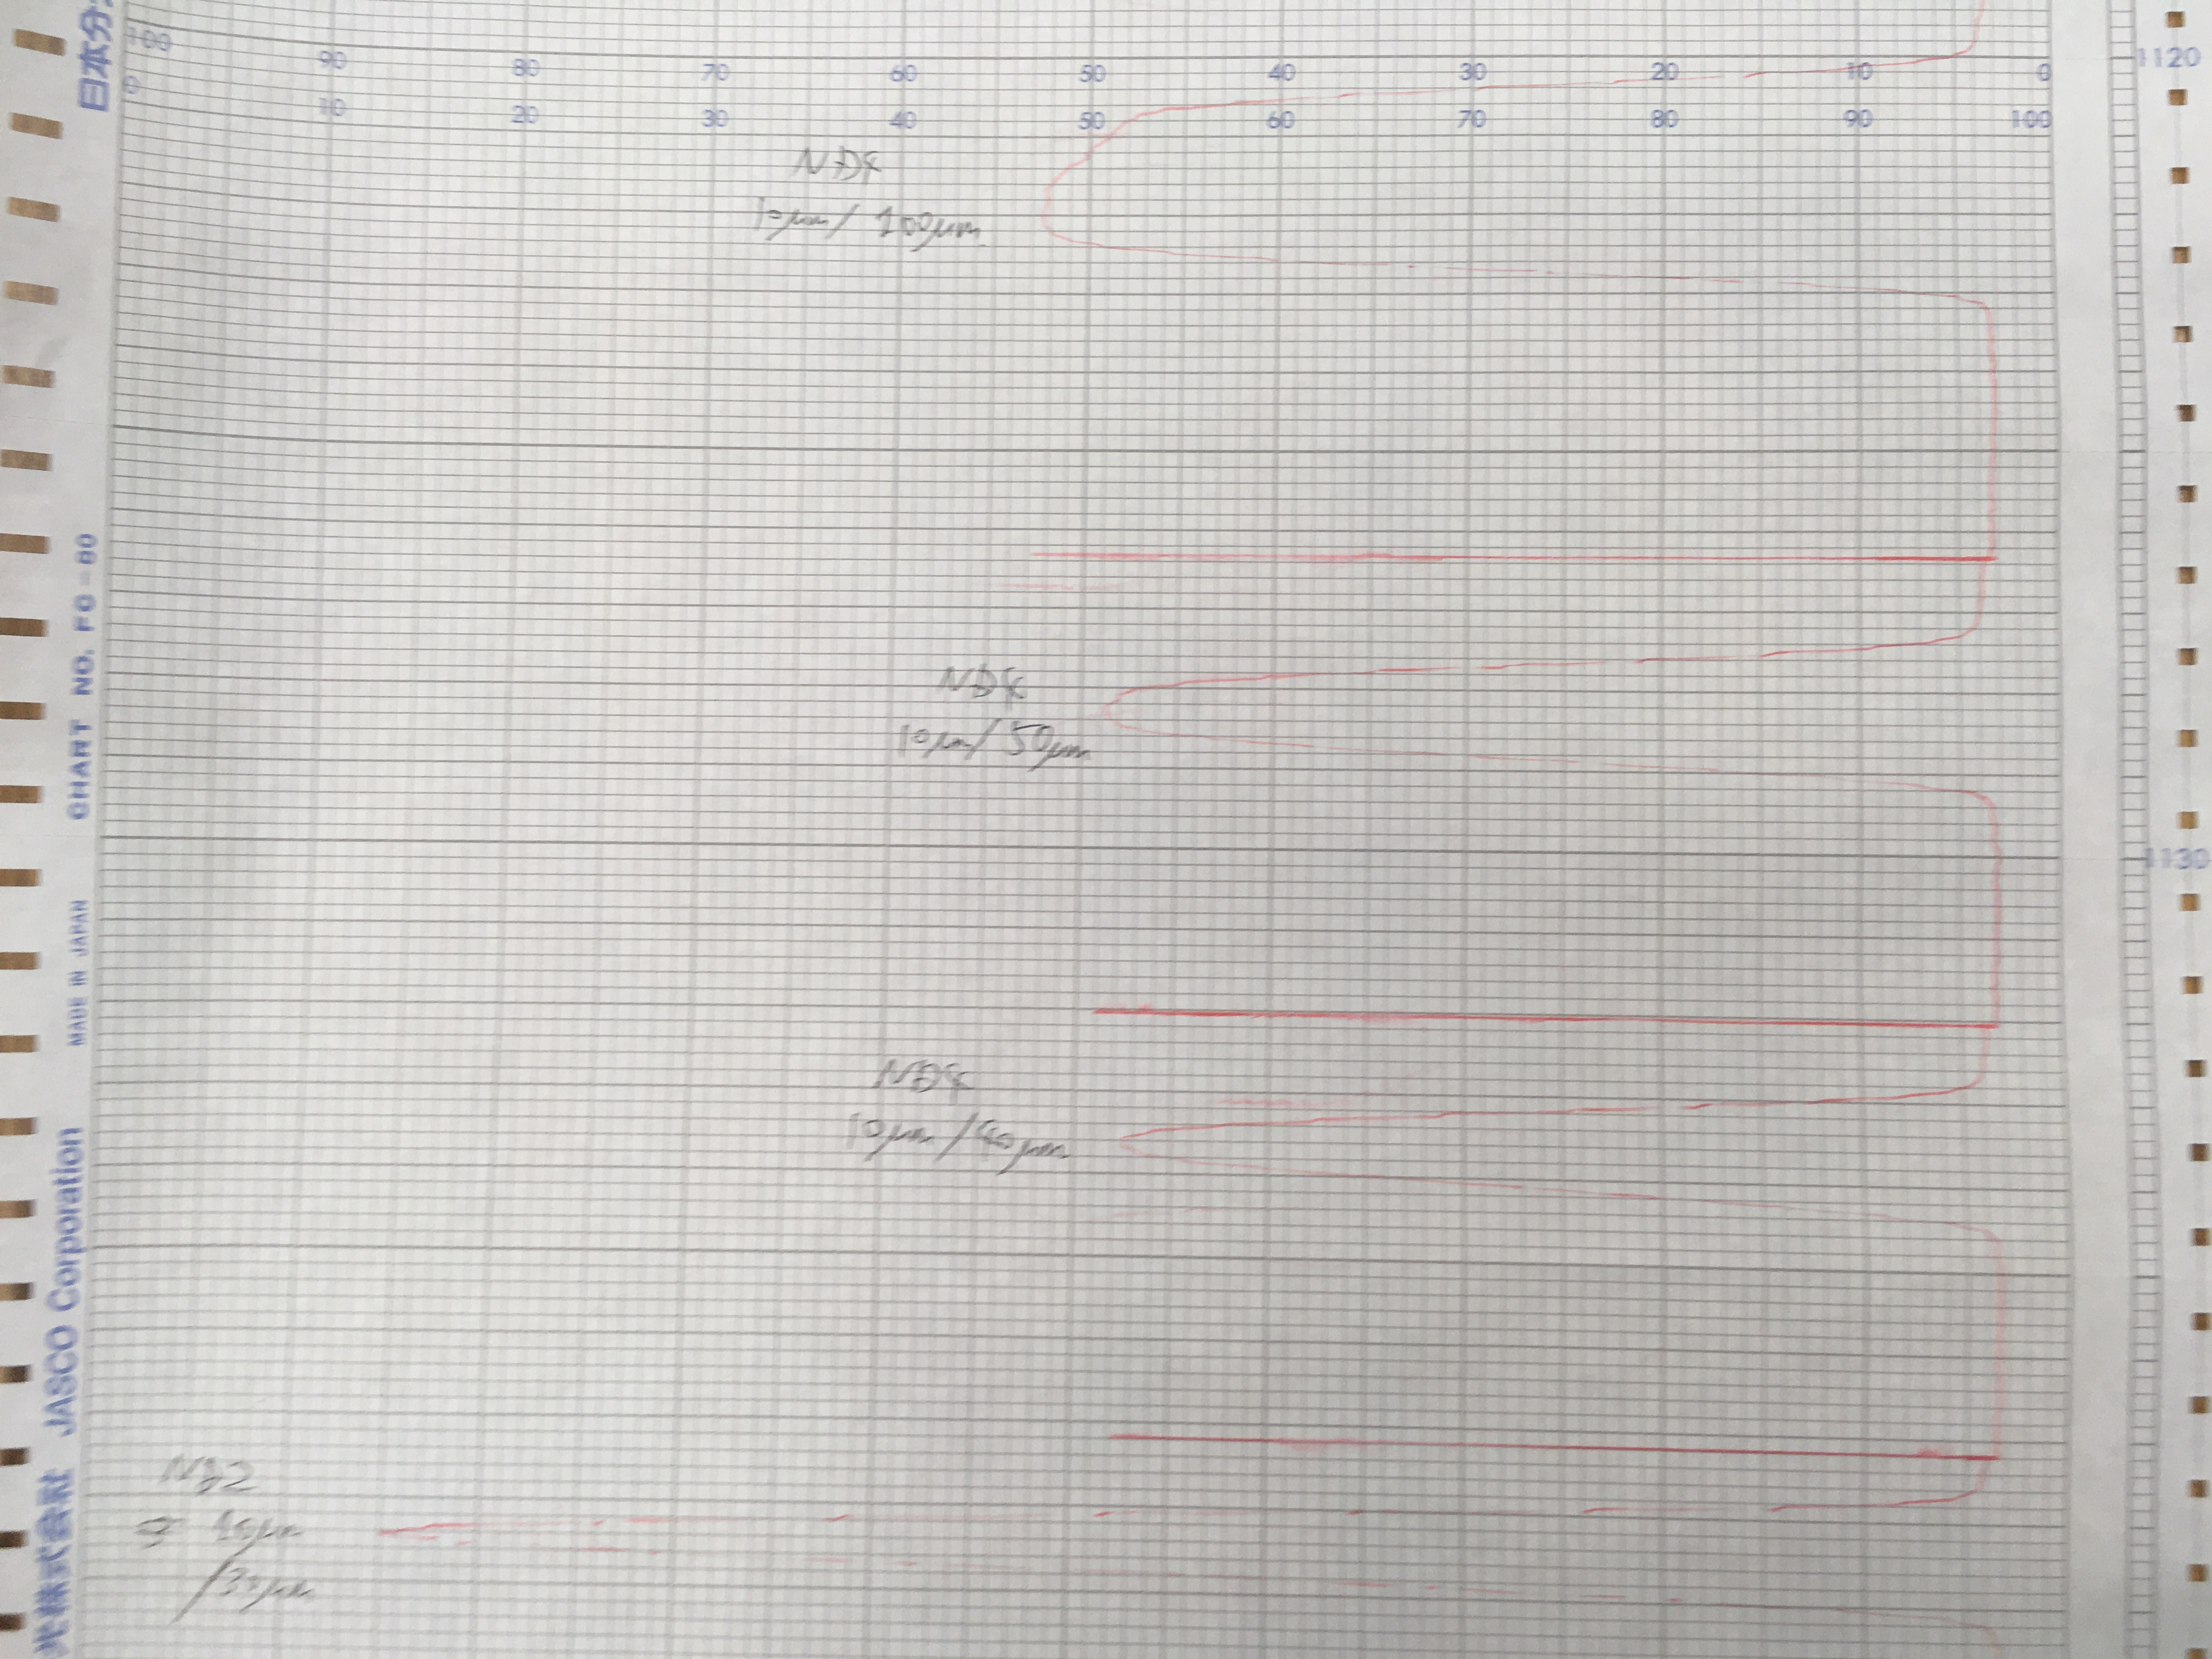
\includegraphics[width=10cm]{d3_delta30-100.JPG}
  \caption{スリットを\SI{100}{\um}開いたときのスペクトル(図上部).図の通り,このスペクトルは台形状だった.}
  \label{fig:daikei}
\end{figure}

また,スリットを\SI{100}{\um}以上開いたときスペクトルは台形状になった(図\ref{fig:daikei}).
本題とは外れるが,これについても考察した.

\subsubsection{考察}
まず,スリット幅とスペクトル幅が比例関係にあると考えられる,図\ref{fig:spectrum_width}左から5番目以降のデータについて,線形フィッティングを行った.
その結果,フィッティング直線は傾き$2.84\pm 0.04$,y切片$0\pm 5$となった.
このことから,確かにスリット幅$\Delta x$の大きいところではほぼ$\Delta \lambda \propto \Delta x$となっており,その比例定数,つまり分散は\SI[separate-uncertainty]{2.84\pm 0.04}{\nm\per\mm}であることが分かる.

次に,ここで得られた結果を,分光器の分散および分解能(解説書図3)と比較する.
まず分光器の分散は約\SI{3}{\nm\per\mm}と記載されているが,これは先ほどのフィッティングから得た分散の値\SI[separate-uncertainty]{2.84\pm 0.04}{\nm\per\mm}と整合する.
また,分解能は半値幅\SI{0.1}{\nm}と記載されているが,これは$\Delta x$が十分小さいときの$\Delta \lambda$の値\SI{60}{\pm}~\SI{70}{\pm}と整合する.
以上より,確かにマニュアルから予想される通りの測定結果が得られたことが確認できた.

最後に,スリットを\SI{100}{\um}以上開くとスペクトルが台形状になったことについて考察する.
これは,分光器の読み取る波長が少し変わっても光の強度がほとんど変わらないことを意味する.
よって,出射スリット上での光のスポット径が出射スリットの幅よりも小さくなっていると考える.
このとき,分光器の回折格子が少し回転しても,光のスポットは出射スリットの内側で動くだけなので,光量は変わらなくなる.
これによって,光のスポット全体が出射スリットに入り込んだ時点で光量は頭打ちとなり,スペクトルはピークの潰れた台形状になる.

ここで,入射スリット幅を広げると出射スリット上でスポット径が狭まることを仮定したが,最後にこれが妥当であることを示す.
本来であればツェルニ-ターナー型分光器の機構から説明すべきだが,ここでは簡単に実験結果から示す.
出射スリット上でのスポットは波長ごとに分解された後のものなので,そのスポット径が小さいことは,スペクトル幅分の波長域がその狭い領域に集まっていることを意味する.
つまり,このとき広い波長域の光が出射スリットに入り込むため,分光器の波長分解能は大きいといえる.
一方,図\ref{fig:spectrum_width}に示したように,入射スリット幅を広げると観測されるスペクトル幅は広くなる.
これは波長分解能が大きいことを意味し,今の考察と合致する.
したがって,入射スリット幅を広げると出射スリットでスポット径が狭まるという説明は妥当であると考える.

\subsection{課題(e)}
ここでは,より分解能を高めた実験を行うためにどうすれば良いか考察する.
まず,分光器の波長分解能は課題(d)で確かめた通り約\SI{0.1}{\nm}である.
そのため,スリット幅を狭くすることで実現できる,一回一回の測定の分解能はこの\SI{0.1}{\nm}より小さくできない.

しかし,$n$回同じ測定を繰り返してその平均をとることで,平均の誤差をもとの$1/\sqrt{n}$倍にすることができる.
そのため,測定の回数を増やすことで,より分解能の高い実験が可能になると考える.
ただし,この測定が意味を持つためには,波長の再現性がある程度必要であることに注意を要する.

\subsection{課題(f)}
ここでは,ペンレコーダーの代わりにコンピューターを用いてスペクトルを記録した.
これ以降の実験では,データ取得はコンピューターを用いて行った.

\subsubsection{手法}
まず,電流電圧変換増幅器の出力をローパスフィルターに入力し,ローパスフィルターの出力をADコンバーターの1番端子に入力した.
これにより,コンピュータ上で分光器の波長を操作できるようになる.
次に,スキャンスピードを\SI{60}{\nm\per\min},スキャンステップを\SI{0.02}{\nm}とし,スキャン範囲を\SI{434}{\nm}から\SI{436}{\nm}までと設定した.
また,入射・出射スリットの幅はともに\SI{10}{\um}とした.
その後,ローパスフィルターの時定数を\SI{2}{\ms},\SI{200}{\ms},throughの3通りに切り替えて,それぞれの場合について測定を行った.

\subsubsection{結果と考察}

\begin{figure}[htbp]
  \centering
  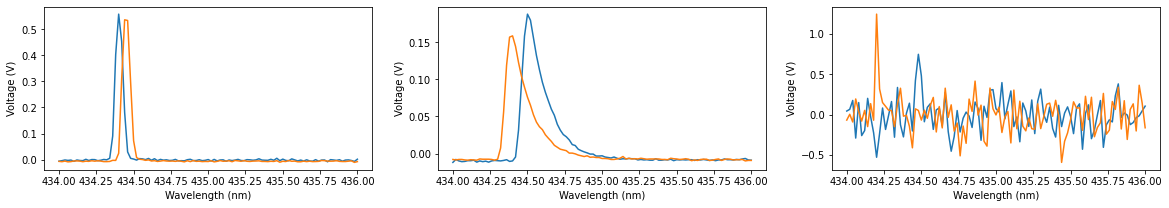
\includegraphics[width=15cm]{amp.png}
  \caption{左から順に,ローパスフィルターの時定数\SI{2}{\ms},\SI{200}{\ms},throughとしたときの測定結果.1回目の測定は青色で,2回目の測定はオレンジ色で示した.}
  \label{fig:amp}
\end{figure}

まず,ローパスフィルターの時定数が\SI{2}{\ms}のとき,図\ref{fig:amp}左のように,課題(c)で見られたような対称なピークが確認できた.

次に,ローパスフィルターの時定数が\SI{200}{\ms}のとき,図\ref{fig:amp}中央のように,長波長側に尾を引いたピークが確認できた.
これは,大きな光電流が長い時定数で平均化されるため,一度生じたピークの影響がしばらく残ったためと考える.

最後に,ローパスフィルターをthroughの設定にしたとき,図\ref{fig:amp}右のように,ピークがノイズに埋もれてしまった.
この場合,信号がまったく平均化されないため,ノイズがそのまま残ってしまったと考える.

\subsection{課題(g)}
\subsubsection{手法}
入射・出射スリットの幅をそれぞれ\SI{20}{\um},\SI{25}{\um}とした.
そして,スキャン範囲を\SI{300}{\nm}から\SI{900}{\nm}までと設定した.
その結果得られたスペクトルから輝線のピーク波長を求め,それと水銀のスペクトル線の文献値から,分光器の波長の較正を行った.
具体的には,分光器の波長の読み$\lambda_{\mathrm{obs}}$と実際の波長$\lambda_{\mathrm{real}}$について
\begin{equation}
  \lambda_{\mathrm{real}} = a \times \lambda_{\mathrm{obs}} + b
\end{equation}
というフィッティングを行い,係数$a,b$を求めた.
最後に,再現性を確かめるため,同じ実験をもう一度行った.

\subsubsection{結果}

\begin{figure}[htbp]
  \centering
  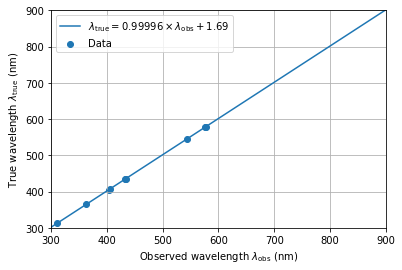
\includegraphics[width=10cm]{lambda_calib.png}
  \caption{波長の較正}
  \label{fig:lambda_calib}
\end{figure}

フィッティングの結果,係数$a,b$は
\begin{align}
  a &= 0.99996 \pm 0.00010 \\
  b &= \SI[separate-uncertainty]{1.69 \pm 0.05}{\nm}
\end{align}
と求まった.
一方,2回目の実験結果をもとにフィッティングを行うと,
\begin{align}
  a &= 0.99983 \pm 0.00008 \\
  b &= \SI[separate-uncertainty]{1.53 \pm 0.04}{\nm}
\end{align}
と求まった.
この結果から,係数$b$は実験するたびに少なくとも0.2程度ゆらぐことが分かる.
このずれをもとに有効数字をとって,以降では次の式で波長を較正する:
\begin{equation}
  \lambda_{\mathrm{real}}(\si{\nm}) = \lambda_{\mathrm{obs}}(\si{\nm}) + \SI{1.7}{\nm}  
\end{equation}


\section{二日目:水素原子の発光スペクトル}
ここでは,水素放電管から放出される光を分光器で測定し,スペクトル線の形状を考察した.

\subsection{課題(a)}
\subsubsection{手法}
まず,一日目と同様に分光器の準備を行った.
ただし,水銀アルゴン光源のかわりに水素放電管を用い,そこに\SI{500}{V}の高電圧を印加した.
次に,一日目の課題(f)と同様の操作を行い,コンピューター上で分光器の波長を操作できるようにした.
ただし,水素放電管からの光は,交流電源により\SI{100}{Hz}で振動しているので,これを除去するためにローパスフィルターの時定数を\SI{200}{\ms}とした.
その後,水素のスペクトル線が確認できる波長範囲で測定を行った.
再現性を確認するため,測定は2回行った.

\subsubsection{結果}

\begin{figure}[htbp]
  \centering
  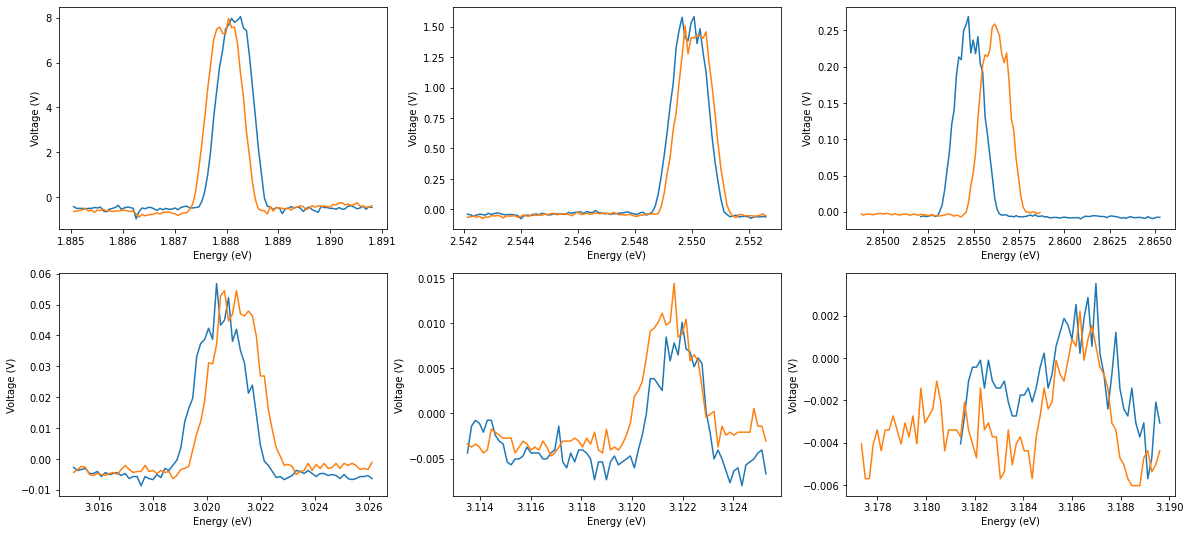
\includegraphics[width=15cm]{Hydrogen.png}
  \caption{水素放電管からの光のスペクトル.ただし青色が1回目;オレンジ色が2回目.横軸にエネルギー(\si{\eV}),縦軸に出力電圧(\si{V})を示した.}
  \label{fig:Hydrogen}
\end{figure}

測定したスペクトルをまとめて図示すると図\ref{fig:Hydrogen}のようになった.
ただし,この図の横軸は波長を較正した値をエネルギーに変換したものである.
これより,高エネルギーのスペクトル線ほどピークの電圧値が小さくなることが分かった.

\subsection{課題(b)}

\begin{figure}[htbp]
  \centering
  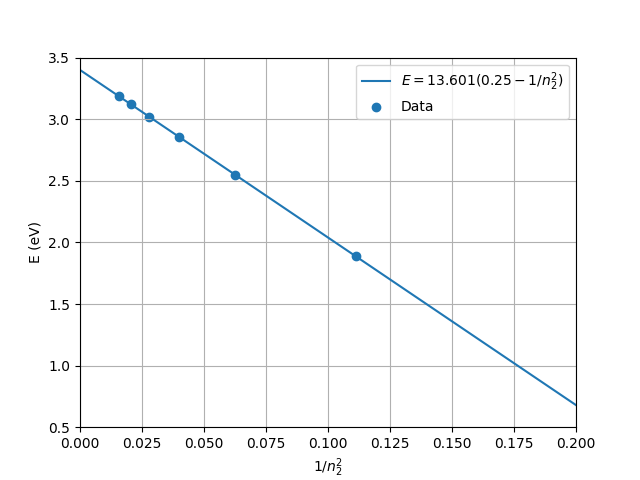
\includegraphics[width=10cm]{balmer_check.png}
  \caption{実験結果がバルマー系列の関係式を満たすことを確認するプロット.縦軸は図\ref{fig:Hydrogen}に示したスペクトルの最大値に対応する波長を較正し,エネルギーに換算したものである.1回目と2回目の実験で得られたピークのエネルギーの差を誤差として考えたが,図においてその誤差棒はプロット点よりも小さかった.}
  \label{fig:balmer_check}
\end{figure}

次式によりフィッティングを行った:
\begin{equation}
  E = R\qty(a - \frac{1}{n_2^2})
\end{equation}
ただし,誤差として1回目と2回目の実験で得たピークのエネルギーの差を用いた.
フィッティングの結果,係数は
\begin{align}
  R &= \SI[separate-uncertainty]{13.601\pm 0.005}{\eV}\\
  a &= 0.24496 \pm 0.00007
\end{align}
と求まった.
それぞれの理論値は$R=\SI{13.6057}{\eV}$,$a=1/4=0.25$であり,これらはフィッティングの誤差の範囲に収まっている.

\subsection{課題(c)}
ここでは,バルマー系列の主量子数$n=3$から$n=2$の遷移で,方位量子数と磁気量子数の遷移が何通りあるかを考える.

まず,主量子数$n=3$となる状態は,方位量子数と磁気量子数の組が
\begin{equation}
  (l,m) = (2, \pm 2), (2, \pm 1), (2, 0), (1, \pm 1), (1, 0), (0, 0)  
\end{equation}
となる場合に限られる.
同様に,主量子数が$n=2$となる状態は,方位量子数と磁気量子数の組が
\begin{equation}
  (l,m) = (1, \pm 1), (1, 0), (0, 0)
\end{equation}
となる場合に限られる.

次に,方位量子数と磁気量子数の遷移には,次に示す選択則がある:
\begin{align}
  \Delta l &= \pm 1 \\
  \Delta m &= 0, \pm 1
\end{align}
つまり,遷移はこの選択則を満たすようにしか起こりえない.

以上より,選択則を満たすような$n=3$から$n=2$への遷移は,表\ref{tab:selection}に示すものに限られる.

\begin{table}[htbp]
  \centering
  \caption{選択則を満たすような$n=3$から$n=2$への遷移}
  \label{tab:selection}
  \begin{tabular}{c|c}
    遷移前の$(l,m)$ & 遷移後の$(l,m)$ \\
    \hline\hline
    (2,2) & (1,1) \\
    (2,1) & (1,1) \\
    (2,1) & (1,0) \\
    (2,0) & (1,1) \\
    (2,0) & (1,0) \\
    (2,0) & (1,-1) \\
    (2,-1) & (1,0) \\
    (2,-1) & (1,-1) \\
    (2,-2) & (1,-1) \\
    \hline
    (1,1) & (0,0) \\
    (1,0) & (0,0) \\
    (1,-1) & (0,0) \\
    \hline
    (0,0) & (1,1) \\
    (0,0) & (1,0) \\
    (0,0) & (1,-1) \\ 
    \hline 
  \end{tabular}
\end{table}

\subsection{課題(d)}

\begin{figure}[htbp]
  \centering
  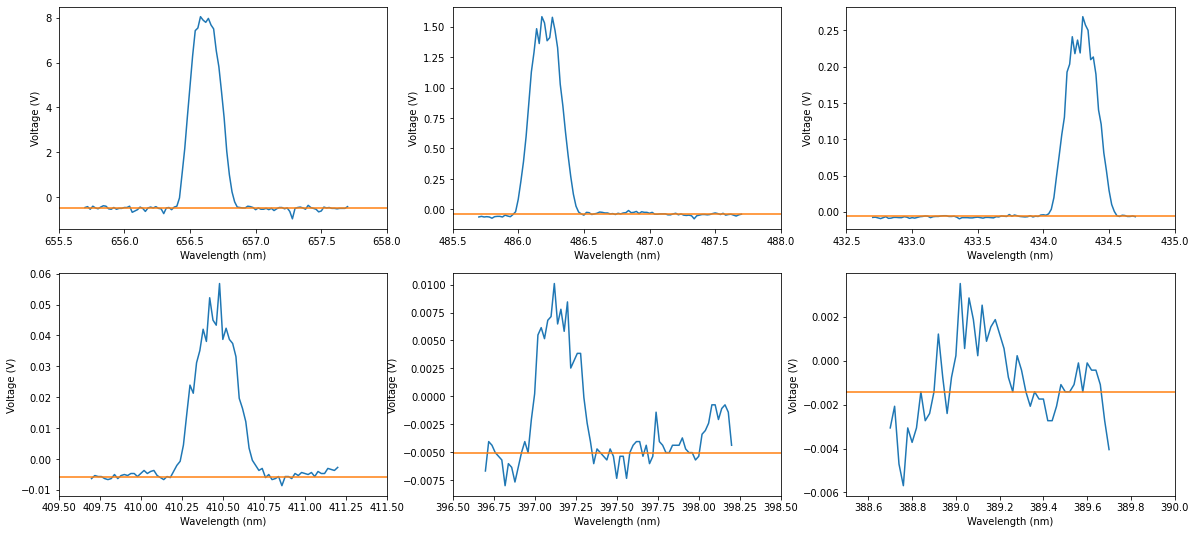
\includegraphics[width=15cm]{intensity_calc.png}
  \caption{課題(c)の1回目の測定で得たスペクトル線(青色)と,その電圧値の最頻値(オレンジ色)との関係.この図から,最頻値をバッグラウンドとして扱うことは概ね正しいと考える.もちろん,この扱い方は$n$が大きくピークが小さくなると疑わしくなるが,本レポートではこの方法で簡単に見積もることにした.}
  \label{fig:intensity_calc}
\end{figure}

ここでは,スペクトル線ごとに発光強度を計算した.
まず,スペクトル線ごとに電圧値の最頻値をとり,これをバックグラウンドと考えた(この推測がそこまで外れていないことは,図\ref{fig:intensity_calc}から確認した.).
次に,電圧値からバックグラウンドを引いた値を測定した波長領域にわたって積分した.
このとき,NDフィルターによって強度の倍率が変わることを考慮し,一日目の課題(b)の表\ref{tab:ND}をもとに,もとの強度を逆算した.
また,積分計算にはシンプトン法を用い,積分範囲はスペクトルの範囲全域にとった.

その結果,図\ref{fig:intensity}のような関係が得られた.
これより,$n=3$からの遷移で発光強度は最大となり,そこから$n$の値が離れるにつれて,強度はほぼ指数的に減少することが分かった.

\begin{figure}[htbp]
  \centering
  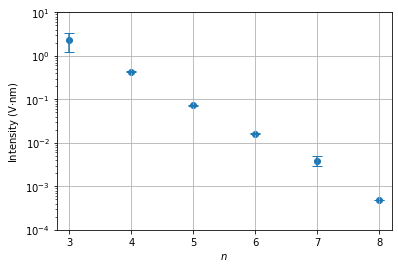
\includegraphics[width=10cm]{intensity.png}
  \caption{スペクトル線の主量子数$n$と発光強度の関係.プロット点は1回目の実験データをもとにした計算結果.誤差棒は1回目と2回目のデータで同じ計算を行って求めた発光強度の差にとった.}
  \label{fig:intensity}
\end{figure}

\subsection{課題(e)}

状態$(n,l)$から状態$(2,l')$への遷移により観測される発光強度$J_{(n,l)}^{(2,l')}$は,磁気量子数$m$の縮重度を考えて
\begin{equation}
  J_{(n,l)}^{(2,l')} = (2l+1)h\nu_{n,l,2,l'} A_{(n,l)}^{(2,l')} \label{trans_intensity}
\end{equation}
と表せると考える.
ただし,$A_{(n,l)}^{(2,l')}, h\nu_{n,l,2,l'}$はそれぞれ遷移確率,遷移エネルギーを表す.
また式\eqref{trans_intensity}では,始状態$(n,l)$がすべての状態にわたって一様分布していると考えている.
水素原子の波動関数の動径成分を$R_{nl}(r)$と書くと,$A_{(n,l)}^{(2,l')}$は$\lvert \int_0^{\infty} r^3 R^{\ast}_{2l'}(r) R_{nl}(r) dr \rvert^2$,つまり状態$(n,l), (2,l')$の波動関数の重なり具合に比例する.
ここで,始状態の$n$が大きくなると,$R_{nl}(r)$の分布は$r$の大きい方向にシフトする.
そのため$n$が2から離れるにつれて,この重なり積分の値は小さくなる.
つまり,$n$を大きくすると遷移確率$A_{(n,l)}^{(2,l')}$は小さくなる.

\begin{figure}[htbp]
  \centering
  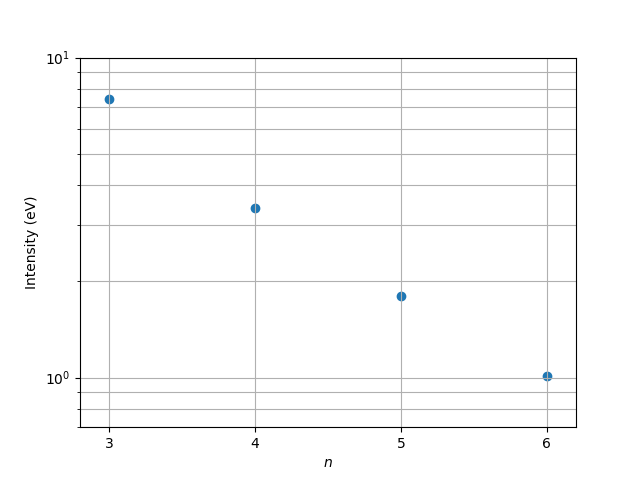
\includegraphics[width=10cm]{intensity_prob.png}
  \caption{発光強度の計算結果}
  \label{fig:intensity_prob}
\end{figure}

また,解説書の図15をもとに,各$n,l,l'$についてこの発光強度$J_{(n,l)}^{(2,l')}$を計算し,$l$について和をとることで$n$ごとの発光強度を求めた.
その結果,図\ref{fig:intensity_prob}のような分布が得られた.
これは,課題(d)で測定結果から得た図\ref{fig:intensity}と同じく,強度が$n$についてほぼ指数的に減少している.
ただし,図\ref{fig:intensity}では,図\ref{fig:intensity_prob}よりも$n$が大きくなったときの強度の減衰が速い.
この違いは,すべての状態$(n,l)$に一様に電子が存在すると考えたことによる.
実際には,高いエネルギー準位に励起される電子は少なくなる\footnote{系が熱平衡にあると見なせばカノニカル分布に従うはずだが,その場合高エネルギー準位にある電子数は少ないことが定量的に分かる.実際には系は非平衡なのでカノニカル分布から外れるが,それでも同様のことが予想される.}ので,$n$が大きい準位からの光の強度は今回のプロット(図\ref{fig:intensity_prob})よりも小さくなると考える.

\subsection{課題(f)}
ここでは,光を放出する水素原子の熱運動に伴うドップラー効果が,スペクトル幅にどれだけ寄与するかを考察する.

まず,温度$T$で熱平衡にある水素原子の速度$v$について,エネルギー等分配則により
\begin{equation}
  \frac{1}{2} \qty(m_e + m_p) \expval{v^2} = \frac{3}{2} k_B T
\end{equation}
が成り立つ.
ただし,$m_e,m_p$はそれぞれ電子,陽子の質量であり,$k_B$はボルツマン定数である.
よって平均二乗速度と光速$c$の比は,
\begin{equation}
  \beta = \frac{\sqrt{\expval{v^2}}}{c} = \sqrt{\frac{3k_B T}{(m_e + m_p)c^2}}
\end{equation}
となる.
よって光のドップラー効果により,波長$\lambda_0$のスペクトルに由来する光の周波数の測定値$f$は,
\begin{equation}
  \sqrt{\frac{1-\beta}{1+\beta}} \le \frac{\lambda}{\lambda_0} \le \sqrt{\frac{1+\beta}{1-\beta}}
\end{equation}
の範囲に広がる.
したがって,$m_p=\SI{1.66e-27}{\kg},m_e=\SI{9.1e-31}{\kg},k_B=\SI{8.62e-5}{\eV\per\kelvin}$を代入すると,$T=\SI{300}{\kelvin}$において,周波数の広がりは
\begin{equation}
  -9.1\times 10^{-6} \le \frac{\lambda-\lambda_0}{\lambda_0} \le 9.1\times 10^{-6}
\end{equation}
と求まる.
今回の実験において,水素原子から観測した波長は$\lambda_0 = \SI{100}{\nm}$のオーダーなので,これに対する周波数の広がりは\SI{1}{\pm}のオーダーとなる.
一方で,分光器の分解能(あるいは実際の測定結果から分かるスペクトル幅)は\SI{0.1}{\nm}のオーダーで,ドップラー効果の寄与の100倍である.
よって,今回の実験で見られたスペクトル幅はドップラー効果によるものではなく,分光器の分解能によるものと考える.

\subsection{課題(g)}
ここでは,スピン軌道相互作用によって水素原子の2p軌道が分裂する効果を考える.
また,この効果によるスペクトルの幅について考察する.

まず,スピン軌道相互作用演算子を表す摂動ハミルトニアンは
\begin{equation}
  \hat{H}'_{\mathrm{SO}} = \frac{\mu_0 Z e^2}{16\pi m_e^2}\frac{1}{r^3} \qty(\hat{\bm{j}}^2 - \hat{\bm{l}}^2 - \hat{\bm{s}}^2)
\end{equation}
で与えられる.
また,原子番号$Z$の水素様原子の場合,2p軌道の動径方向の波動関数は
\begin{equation}
  R_{2,1}(r) = \frac{1}{2\sqrt{6}} \qty(\frac{Z}{a_0})^{\frac{3}{2}} \frac{Zr}{a_0} \exp(-\frac{Zr}{2a_0})
\end{equation}
で与えられる.
これらを用いると,スピン軌道相互作用によるエネルギー固有値の一次の摂動は,
\begin{equation}
  \Delta \varepsilon = \hbar^2 \frac{j(j+1) - l(l+1) - s(s+1)}{2} \frac{\mu_0 Z e^2}{16\pi m_e^2} \expval{\frac{1}{r^3}}{R_{nl}}
\end{equation}
となる.
ここで,
\begin{align}
  \expval{\frac{1}{r^3}}{R_{nl}} &= \int_0^\infty dr\, r^2 \frac{1}{r^3} \frac{1}{24} \qty(\frac{Z}{a_0})^3 \qty(\frac{Zr}{a_0})^2 \exp(-\frac{Zr}{a_0})\notag\\
  &= \frac{1}{24} \qty(\frac{Z}{a_0})^3 \int_0^\infty dx\, x e^{-x} \notag\\
  &= \frac{1}{24} \qty(\frac{Z}{a_0})^3 
\end{align}
と計算できるので,$l=1,s=1/2$より,
\begin{align}
  \Delta \varepsilon &= \hbar^2 \frac{j(j+1) - 11/4}{2} \frac{\mu_0 Z e^2}{16\pi m_e^2} \frac{1}{24} \qty(\frac{Z}{a_0})^3  \notag\\
  &= \frac{j(j+1) - 11/4}{48} \frac{\mu_0 Z e^2\hbar^2}{16\pi m_e^2} \qty(\frac{Z}{a_0})^3 \notag\\
  &= \left\{
  \begin{array}{ll}
    \frac{1}{48}\frac{\mu_0 Z e^2\hbar^2}{16\pi m_e^2} \qty(\frac{Z}{a_0})^3 & (j = 3/2) \\
    -\frac{2}{48}\frac{\mu_0 Z e^2\hbar^2}{16\pi m_e^2} \qty(\frac{Z}{a_0})^3 & (j = 1/2)
  \end{array}
  \right.
\end{align}
となる.
よって,分裂エネルギー$\Delta$は
\begin{equation}
  \Delta =\frac{1}{16}\frac{\mu_0 Z e^2\hbar^2}{16\pi m_e^2} \qty(\frac{Z}{a_0})^3 \label{split}
\end{equation}
と求まる.
これより,分裂エネルギーは原子番号$Z$の4乗に比例することが分かる.

また,水素原子($Z=1$)の場合について式\eqref{split}を具体的に計算すると,$\Delta \approx \SI{0.023}{\meV}$と求まる.
一方で,波長$\lambda \le \SI{600}{\nm}$の光について,分光器の分解能$\Delta \lambda = \SI{0.1}{\nm}$のために生じるスペクトル幅は,
\begin{equation}
  \Delta E = \frac{hc}{\lambda^2} \Delta\lambda \ge \SI{0.25}{\meV}
\end{equation}
と計算できる.
つまり,分光器の分解能によるスペクトル幅は,スピン軌道相互作用によるスペクトル幅の少なくとも10倍以上である.
よって,今回の実験で見られたスペクトル幅はスピン軌道相互作用によるものではなく,やはり分光器の分解能によるものと考える.

\section{三日目:半導体の透過スペクトル・低温測定}
ここでは,半導体GaAsおよびCu$_2$O試料の分光測定を行った.
この測定結果をもとに,GaAsのバンドギャップエネルギーを見積もった.
また,Cu$_2$Oに生じる励起子を観測した.

\subsection{光学系の準備}
最初に,次の手順に沿って光学系を準備した.

まず,タングステンハロゲンランプを曲面ミラーに当て,その反射光をレンズAに通して集光した.
次に,光の集光位置の後方にレンズBを置き,再び平行光に戻した.
そして,その平行光をミラーA,Bにより2度反射させ,反射光をレンズCに通し,分光器のスリットに集光させた.

以降の実験では,試料の位置はレンズAによる集光位置に固定した.
そのため,この位置を試料位置と呼ぶことにする.

\subsection{課題(a)}
ここでは,半導体GaAsの分光測定を行った.

\subsubsection{手法}
上述した光学系の準備を行った後,入射・出射スリットの幅をともに\SI{100}{\um}に調整した.
まず,試料位置に何も置かずに測定を行った(リファレンス).
次に,試料位置にGaAsを置いて測定を行った(GaAs試料透過光).
最後に,分光器から出てくる光をカットして測定を行った(バックグラウンド).
ただし,2次回折光の影響を防ぐため,約\SI{600}{\nm}以下の波長の光をカットする赤色フィルターを適宜ミラーA,B間に置いた.

\subsubsection{結果}
実験の結果,図\ref{fig:GaAs}のようなスペクトルが得られた.

\begin{figure}[htbp]
  \centering
  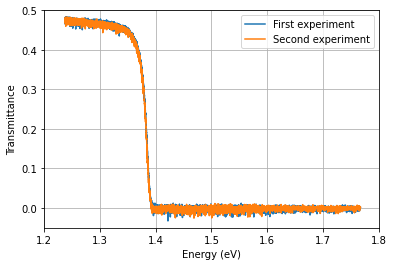
\includegraphics[width=10cm]{GaAs.png}
  \caption{半導体GaAsの透過率.ただし,縦軸をエネルギー透過率,横軸を光子エネルギー(eV)とした.また,1回目の計測結果を青色で,2回目の計測結果をオレンジ色で示した.}
  \label{fig:GaAs}
\end{figure}

\subsection{課題(b)}

課題(a)の図\ref{fig:GaAs}より,1回目(青色)も2回目(オレンジ色)も,エネルギー\SI{1.39}{\eV}付近で急激に透過率が立ち上がることが分かる.
そのため,これをGaAsのバンドギャップエネルギーの測定値と考える.
一方で,テキストp.34の図9より,GaAsのバンドギャップエネルギーの文献値は\SI{1.42}{\eV}である.
つまり,本来のバンドギャップエネルギーよりも約\SI{3}{\meV}だけ小さなエネルギーで立ち上がりが観測されたことになる.
このずれは格子振動や励起子の束縛によるエネルギーよりも大きいため,結晶に何らかの不純物があった可能性が考えられる.

\subsection{課題(c)}
ここでは,半導体Cu$_2$Oの分光測定を行った.

\subsubsection{手法}
まず,半導体GaAsのかわりにクライオスタットを置き,その内部にある半導体Cu$_2$Oが試料位置に来るように調整した.
また,この実験では,NDフィルターは試料の前に置き直した.

次に,入射スリットと出射スリットの幅をともに\SI{50}{\um}とした.
その後,クライオスタットを取り外し,試料位置に何も置かないようにして測定を行った(リファレンス,常温).
次に,クライオスタットを戻して測定を行った(Cu$_2$O試料透過光,常温),
その後,光を遮って測定を行った(バックグラウンド,常温).

次に,クライオスタットに液体窒素を注ぎ,試料を\SI{77}{\kelvin}まで冷却した.
この温度は,クライオスタットの試料付近に設置された白金測温抵抗体の抵抗値をもとにモニターした.
この状況で,再び試料透過光を測定した.
リファレンスとバックグラウンドについては,最初の測定で得たものをそのまま用いた.

最後に,クライオスタットのヒーターをONにし,試料の温度を\SI{150}{\kelvin}にして,再び試料透過光を測定した.

\subsubsection{結果と考察}
\begin{figure}[htbp]
  \centering
  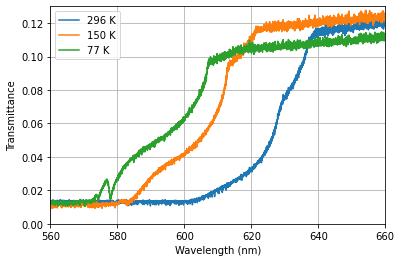
\includegraphics[width=10cm]{Cu2O_transmittance.png}
  \caption{半導体Cu$_2$Oの透過スペクトル.縦軸にエネルギー透過率,横軸に光の波長をとった.}
  \label{fig:Cu2O_transmittance}
\end{figure}

\begin{figure}[htbp]
  \centering
  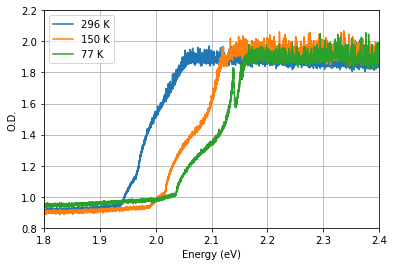
\includegraphics[width=10cm]{Cu2O_OD_c.png}
  \caption{半導体Cu$_2$Oの吸収スペクトル.縦軸に光学密度(O.D.),横軸に光のエネルギーをとった.}
  \label{fig:Cu2O_OD_c}
\end{figure}

実験の結果,図\ref{fig:Cu2O_transmittance}のような透過スペクトルが得られた.
これより,立ち上がりはGaAsのときと比べて緩やかであり,温度が高くなるにつれて透過スペクトルの立ち上がりが長波長側(低エネルギー側)にシフトしていることが分かった.
また,\SI{77}{\kelvin}でのみ,波長\SI{580}{\nm}付近に小さな吸光ピークが見られた.
また,透過率を光学密度に,光の波長をエネルギーに換算すると,図\ref{fig:Cu2O_OD_c}のようになった.

次に,温度が高くなるにつれて透過スペクトルの立ち上がりが低エネルギー側にずれたことについて考察する.
本来,半導体内のバンドは固定的なものではなく,格子振動など熱の影響でゆらいでいる.
このゆらぎは温度とともに激しくなるので,高温ではバンドのエネルギー準位は大きくゆらぐことになる.
そのため,高温では本来のバンドギャップよりも小さなエネルギーの光でも,バンド間遷移が起こる可能性がある.
また,その可能性は温度が上がるにつれて大きくなる.
したがって,本来のバンドギャップよりも小さなエネルギーでのバンド間遷移が目立つ高温では,立ち上がりが低エネルギーにシフトしたと考える.

この結果のその他の部分については,以降の課題で考察する.
たとえば,立ち上がりが緩やかであったことについては,課題(e)で考察する.
また,\SI{77}{\kelvin}で見られた小さな吸光ピークについては,課題(d)で背景となる理論を述べた後,課題(e)で考察する.
さらに課題(f),(g)では,追加実験の結果をもとにより詳細な議論を行う.

\subsection{課題(d)}
\subsubsection{励起子束縛エネルギー}
ここでは,Cu$_2$Oの励起子束縛エネルギーを求める.
まず,電子質量を$m_e$とすると,Cu$_2$Oの低エネルギー側の伝導体の電子の有効質量は$m^*_e = 0.99m_e$,高エネルギー側の価電子帯の正孔の有効質量は$m^*_h = 0.58m_e$である.
よって,電子と正孔の換算質量は
\begin{equation}
  \mu^* = \qty(\frac{1}{m^*_e} + \frac{1}{m^*_h})^{-1} = 0.366 m_e
\end{equation}
と求まる.
一方,励起子のエネルギー系列は,自然数$n$を用いて
\begin{equation}
  E_n^{\mathrm{ex}} = \frac{\mu^*}{m_e}\frac{1}{\varepsilon_r^2} E_n
\end{equation}
と書ける.
ただし,$\varepsilon_r$は比誘電率であり,今回は$\varepsilon_r=7.3$とする.
また,$E_n$は水素原子のエネルギー系列であり,次式で与えられる:
\begin{equation}
  E_n = -\frac{R}{n^2}
\end{equation}
ここで,$R=\SI{13.7}{\eV}$はリュードベリ定数である.
以上より,
\begin{equation}
  E_n^{\mathrm{ex}} = -\frac{\mu^*}{m_e}\frac{1}{\varepsilon_r^2} \frac{R}{n^2} = -\frac{\SI{93.3}{\meV}}{n^2}
\end{equation}
がいえる.

\subsubsection{励起束縛エネルギーの温度換算と励起子Bohr半径}
次に,$n=1,4$の場合について,先ほど求めた束縛エネルギーを熱エネルギー$k_BT_n$に対応させたときの温度$T_n$を求める.
ただし,$k_B=\SI{8.6217e-2}{\meV\per\kelvin}$はボルツマン定数である.
計算の結果,
\begin{align}
  T_1 = \frac{\lvert E_1^{\mathrm{ex}}\rvert}{k_B} &= \SI{1.08e3}{\kelvin} \\
  T_4 = \frac{\lvert E_4^{\mathrm{ex}}\rvert}{k_B} &= \SI{43.3}{\kelvin}
\end{align}
となる.

また,水素原子との類推から,励起子のBohr半径は
\begin{equation}
  a_B = \frac{\varepsilon_r m_e a_H}{\mu^*} = \SI{1.06}{\nm}
\end{equation}
と考えられる.
ただし,$a_H=\SI{0.053}{\nm}$は水素原子のBohr半径である.

\subsection{課題(e)}
Cu$_2$Oの励起子の光吸収は,最低エネルギーとして1s状態,2s状態ではなく,2p状態が観測される.
ここではこの理由を考察する.

まず,Cu$_2$Oは直接遷移型半導体(価電子帯の頂点と伝導帯の頂点が同じ波数を持つ半導体)である.
そして,価電子帯はCu原子の4d軌道からなり,伝導帯はCu原子の4s軌道からなる.
ここで,各バンドのパリティを考えると,価電子帯も伝導帯も偶パリティを持つことが分かる.
そのため遷移が起こっていないもとの状態および励起子の1s状態,2s状態は偶パリティとなり,2p状態ではじめて奇パリティとなる.
ここで,電気双極子近似の下では,パリティを変えない遷移が光学禁制であることが知られている.
つまり,もとの状態から励起子の1s状態と2s状態への遷移は,偶パリティから偶パリティへの遷移なので,これは光学禁制であり基本的には実現しない.
一方で,もとの状態から励起子の2p状態への遷移は,偶パリティから奇パリティへの遷移なので,これは光学許容であり実現する.

以上の議論をもとに,課題(c)で得られたCu$_2$Oの透過スペクトルの立ち上がりが,GaAsと比べて緩やかであったことを考察する.
まずGaAsの場合,$\Gamma$点において価電子帯は主に4s軌道からなり,伝導体は4p軌道からなる.
そのため,GaAsのバンド間遷移は偶パリティから奇パリティへの遷移となり,光学許容である.
一方でCu$_2$Oのバンド間遷移は,偶パリティから偶パリティへの遷移なので,光学禁制である.
したがって,$Cu_2O$のバンド間遷移は電気双極子以外の遷移またはフォノンによる間接遷移となるので,光のエネルギーがバンドギャップに近づいても急激には吸光しない.
そのため,Cu$_2$Oのスペクトルの立ち上がりが緩やかになると考える.

\subsection{課題(f)}
ここでは,半導体Cu$_2$Oの励起子の4p状態と5p状態を観測するため,再び低温で分光測定を行った.

\subsubsection{計測に必要な波長分解能の導出}
課題(d)の計算により,Cu$_2$Oの励起子の4p状態および5p状態の束縛エネルギーはそれぞれ\SI{5.83}{\meV},\SI{5.73}{\meV}と求まる.
また,Cu$_2$Oの価電子帯と伝導帯のバンドギャップエネルギーの文献値は\SI{2.17}{\eV}である.
そのため,価電子帯と伝導帯に一組の正孔と電子を作り,それを4p状態として束縛するのに要するエネルギーは\SI{2.1642}{\eV}と求まり,また5p状態として束縛するのに要するエネルギーは\SI{2.1663}{\eV}と求まる.
よって,これらの遷移の際に吸収する波長はそれぞれ\SI{572.88}{\nm},\SI{572.32}{\nm}と見積もられる.
したがって,この波長を見分けるには,波長分解能として約\SI{0.56}{\nm}が必要である.

この波長分解能を実現するため,スキャンスピードを\SI{5.00}{\nm\per\min},スキャンステップを\SI{0.05}{\nm}に変更し,さらにコンピュータへの読み込み速度を変えることで,時定数を\SI{200}{\ms}とした.

\subsubsection{手法}
引き続き,入射スリットと出射スリットの幅をともに\SI{50}{\um}とした.
その後,クライオスタットの温度を\SI{77}{\kelvin}として,課題(c)と同様の測定を行った.

\subsubsection{結果と考察}

\begin{figure}[htbp]
  \centering
  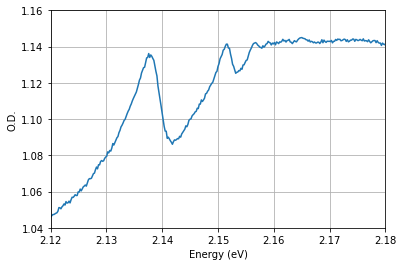
\includegraphics[width=10cm]{Cu2O_4p5p.png}
  \caption{温度\SI{77}{\kelvin}における半導体Cu$_2$Oの吸収スペクトル.縦軸に光学密度,横軸にエネルギーをとった.}
  \label{fig:Cu2O_4p5p}
\end{figure}

得られた計測結果をもとに,波長をエネルギーに,スペクトルの強度を光学密度に変換すると,図\ref{fig:Cu2O_4p5p}のような吸収スペクトルとなった.
これより,約\SI{2.138}{\eV}をはじめとする吸収ピークが複数みられることが分かった.

これまでの考察から,ここで見られたピークは,Cu$_2$Oに励起子が生じることによるものと考える.
さらに課題(e)の議論から,Cu$_2$Oの場合,エネルギーの低い順に2p.3p,4p,5p状態の励起子が生じることが分かる.
そこで,得られた吸収ピークのエネルギーとこの励起子の状態を対応づけると,表\ref{tab:Cu2O_4p5p}のようになった.
ただし,吸収ピークのエネルギーとして,ピークの極大点におけるエネルギーを採用した.
また,スペクトルからの確認が難しかった6p以降の状態については割愛する.
この表\ref{tab:Cu2O_4p5p}から,理論値と測定値の間に\SI{7}{\meV}~\SI{10}{\meV}程度の差があることが読み取れる.
このずれは,ピークの形状がファノ共鳴により左右が非対称となり,極大点が必ずしも準位間のエネルギーに対応しないことによるものと考える.
ただし,たとえば励起子の2p状態への遷移エネルギーの理論値の示す位置を図\ref{fig:Cu2O_4p5p}で確認すると,まったくピークの見られない領域にあることが読み取れるので,この考察は疑問が残る.

\begin{table}[htbp]
  \centering
  \caption{励起子の状態と,その状態への遷移に必要なエネルギーの関係.}
  \label{tab:Cu2O_4p5p}
  \begin{tabular}{cc|c}
    励起子の状態 & 理論値(\si{\eV}) & 測定値(\si{\eV}) \\
    \hline\hline
    2p & 2.1467 & 2.1376 \\
    3p & 2.1596 & 2.1515 \\
    4p & 2.1642 & 2.1567 \\
    5p & 2.1663 & 2.1590 \\
    \hline
  \end{tabular}
\end{table}


\subsection{課題(g)}

これ以降の課題について,テキストでは課題(f),(g),(h)とあったが,課題(f)が重複してしまうので,本レポートではそれぞれ課題(g),(h),(i)と書き直した.

\begin{figure}[htbp]
  \centering
  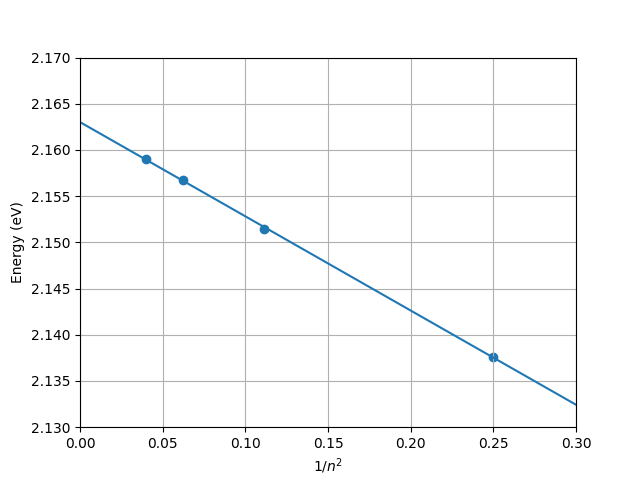
\includegraphics[width=10cm]{excitons.png}
  \caption{励起子の束縛状態の量子数を$n$としたとき,$1/n^2$とその束縛状態への遷移エネルギーの関係.}
  \label{fig:excitons}
\end{figure}

表\ref{tab:Cu2O_4p5p}に示した,励起子の主量子数$n$とその状態への遷移に必要なエネルギー$\Delta E_n$は,理論的には次式に従って決まる:
\begin{equation}
  \Delta E_n = E_g + E_n^{\mathrm{ex}} = E_g - R'\frac{1}{n^2} \label{EgR_fit}
\end{equation}
ただし,バンドギャップエネルギーは$E_g = \SI{2.17}{\eV}$であり,係数$R'$は
\begin{equation}
  R' = \frac{\mu^*}{m_e}\frac{1}{\varepsilon_r^2} R = \SI{0.0934}{\eV}
\end{equation}
である.
そこで,式\eqref{EgR_fit}を$E_g,R'$をパラメータとする$1/n^2$に関する関数と考え,これをもとにフィッティングを行った.
フィッティングの結果,
\begin{align}
  R' = \SI[separate-uncertainty]{0.1019 \pm 0.0010}{\eV} \\
  E_g = \SI[separate-uncertainty]{ 2.16302 \pm 0.00013}{\eV}
\end{align}
と求まった.
これと$R',E_g$の理論値,文献値を比較すると,値としては近いものの,フィッティングの誤差以上に離れていることが分かる.
これは,課題(f)で述べた通り,ここで用いたエネルギーの値はファノ共鳴を考慮していないので不正確であるためと考える.

\subsection{課題(h)}

ここでは,励起子吸収ピークのエネルギー幅と励起子の主量子数$n$の関係を考察する.

まず,励起子吸収ピークのエネルギー幅$\Delta E$は,エネルギーと時間の不確定性関係から,
\begin{equation}
  \Delta E \sim \frac{\hbar}{\Delta t}
\end{equation}
となる.
ただし,$\Delta t$は励起子状態の寿命である.
ここで,励起子のnp状態から1s状態への遷移確率は$(n-1)^2/n^5$に従うことが予想されるので,$\Delta t$はその逆数に比例すると考える.
よって比例定数を$a$として
\begin{equation}
  \Delta E = a \frac{(n-1)^2}{n^5} \label{energy_width}
\end{equation}
が成り立つと考える.

\begin{figure}[htbp]
  \centering
  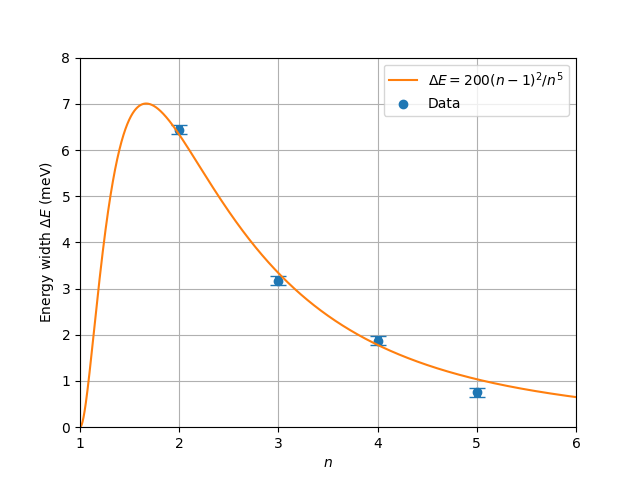
\includegraphics[width=10cm]{Cu2O_energy_width.png}
  \caption{励起子の量子数$n$と励起子吸収ピークのエネルギー幅$\Delta E$の関係.オレンジ色の曲線は式\eqref{energy_width}の形でフィッティングを行って得られたものである.また,誤差棒はスペクトルのデータの刻み幅の半分である\SI{0.1}{\meV}の大きさにとった.}
  \label{fig:Cu2O_energy_width}
\end{figure}

次に,今回の実験結果をもとに励起子吸収ピークのエネルギー幅を求めた.
そのために,まず図\ref{fig:Cu2O_4p5p}に示したスペクトルの各吸収ピークに対してバックグラウンドと思われる直線を引いた.
次に,スペクトルとその直線との差をとって再度プロットした.
最後に,この新しいプロットをもとにピークの半値全幅を求め,それをエネルギー幅$\Delta E$とした.

以上の操作によって得た$\Delta E$を式\eqref{energy_width}とともにプロットすると,図\ref{fig:Cu2O_energy_width}のようになった.
ただし,誤差棒は取得したスペクトルのデジタルデータの刻み幅(エネルギー間隔,約\SI{0.2}{\meV})の半分である\SI{0.1}{\meV}にとった.
これは,半値全幅を求めるときに差をとった二つのデータ点のエネルギーの誤差を表している.
また,式\eqref{energy_width}の形でフィッティングを行った結果,$a=200\pm 30$と求まった.
そのフィッティング曲線も図\ref{fig:Cu2O_energy_width}に示した(オレンジ色).
これより,確かに式\eqref{energy_width}は実験結果をよく説明していることが分かる.
$n=5$のデータ点が曲線からやや外れているのは,ピークが小さかった(ピークを構成するデジタルデータの数が少なかった)ため,バックグラウンドの直線や半値全幅が不正確だったためと考える.

\subsection{課題(i)}
ここでは,Cu$_2$Oの1s励起子による吸収スペクトルを測定した.

\begin{figure}[htbp]
  \centering
  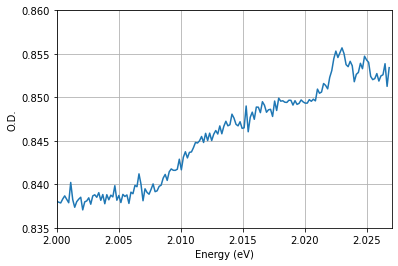
\includegraphics[width=10cm]{Cu2O_1s.png}
  \caption{温度\SI{77}{\kelvin}における1s励起子の吸収スペクトル.}
  \label{fig:Cu2O_1s}
\end{figure}

測定は課題(f)とまったく同様に行った.
その結果,図\ref{fig:Cu2O_1s}のようなスペクトルが得られた.
これより,約\SI{2.023}{\eV}のエネルギーに吸収ピークが確認できた.
これを1s励起子への遷移エネルギーの測定値と考える.
この吸収ピークの位置とCu$_2$Oのバンドギャップの大きさの文献値\SI{2.17}{\eV}ことから,1s状態の励起子の束縛エネルギーは\SI{153}{\meV}と求まる.

ここでまず,1s状態の励起子の準位への遷移がなぜ起こるかを考察する,
課題(e)で議論したように,双極子近似の下ではパリティを変えない遷移は光学禁制となる.
つまり,もとの状態から1s励起子の準位への遷移は,偶パリティから偶パリティへの遷移なので,光学禁制となる.
ところが,Cu$_2$Oの場合,奇パリティのフォノンを吸収・放出しながら1s励起子の準位へ光学遷移する.
この過程は光学許容となるので実現する.

また,課題(d)の方法で計算される1s状態の励起子の束縛エネルギーは約\SI{93.4}{\meV}である.
これは実験で得た値とかなりかけ離れている.
これはCu$_2$O内にできた電子と正孔が,水素原子の電子と原子核のように自由に動くわけではないことに起因する.
課題(d)で求めたように,励起子のBohr半径は\SI{1.06}{\nm}である.
これは半導体Cu$_2$Oの格子定数と同程度なので,電子と正孔はある原子核まわりに局在することになる.
したがって,水素原子モデルから計算した束縛エネルギーは実際とは異なると考える.

\section{感想}
本実験を通して,光と物質の相互作用について今までより深く理解できました.
「準位間のエネルギー差に対応する光が吸収・放出される」という,一見常識のような知識を裏付ける物理に初めて触れることができ,その上で実験できたことは幸運だったと思います.
実験の原理を数式でしっかりと理解するのはやや難しかったですが,実験を監督してくださった方の説明が分かりやすかったので,直観的には理解できました.
また,半導体Cu$_2$Oを用いることで,大きな$n$まで励起子を見ることができて面白かったです.

改善点を挙げるとすれば,ペンレコーダーのペンが何度も外れて実験をやり直すことになったので,調整していただけると実験がよりスムーズになると思います.
また,実験で用いた試料の厚みを測定しましたが,そのデータの使いどころがよく分かりませんでした.
このデータを用いる必要のある課題は見つからなかったので,もしこれをもとに考察できる部分がありましたら,解説書に追記していただければ嬉しいです.

\begin{thebibliography}{99}
  \bibitem{text}
    「物理学実験\ajRoman{2}」解説書「分光測定」2021年度
\end{thebibliography}

\end{document}